\documentclass[11pt,pdf,hyperref={unicode}]{beamer}
%\usetheme{boxes}
\beamertemplatenavigationsymbolsempty
\setbeamertemplate{footline}[page number]
% Set it for the internal PhD thesis defence to reduce number of slides
%\setbeamersize{text margin left=0.5em, text margin right=0.5em}

\usepackage[utf8]{inputenc}
%\usepackage[english, russian]{babel}
\usepackage{bm}
\usepackage{multirow}
\usepackage{ragged2e}
\usepackage{indentfirst}
\usepackage{multicol}
\usepackage{subfig}
\usepackage{amsmath,amssymb}
\usepackage{enumerate}
\usepackage{mathtools}
\usepackage{comment}
\usepackage[all]{xy}
\usepackage{tikz}
\usetikzlibrary{positioning,arrows}
\tikzstyle{name} = [parameters]
\definecolor{name}{rgb}{0.5,0.5,0.5}

%\usepackage{caption}
%\captionsetup{skip=0pt,belowskip=0pt}

%\newtheorem{theorem}{Theorem}
%\newtheorem{statement}{Statement}
%\newtheorem{definition}{Definition}

% colors
\definecolor{darkgreen}{rgb}{0.0, 0.2, 0.13}
\definecolor{darkcyan}{rgb}{0.0, 0.55, 0.55}
%\AtBeginEnvironment{figure}{\setcounter{subfigure}{0}}
%\captionsetup[subfloat]{labelformat=empty}

%----------------------------------------------------------------------------------------------------------

\title{Cover Success Predictor: Enhancing Book Cover Design with Machine Learning}
%\author{Name Surname}
%\institute[]{}
%\date{2024}

%---------------------------------------------------------------------------------------------------------
\begin{document}
%\begin{frame}
%\titlepage
%\end{frame}
    \setcounter{page}{2}%remove here for the title
%----------------------------------------------------------------------------------------------------------
%\section{Please do not use sectioning in the presentations}
    \begin{frame}{Cover Success Predictor: Maximizing Book Cover Impact}
        In an increasingly digital world, first impressions are critical for book success.

        \begin{block}{The problem}
            To investigate the optimization of book cover designs for attracting initial reader engagement in a competitive online marketplace.
        \end{block}
        \begin{block}{Method}
            Using data analytics and machine learning to predict cover effectiveness based on visual and contextual features.
        \end{block}
        \begin{block}{Contribution}
            Provide an innovative tool that helps authors design more effective book covers, reducing reliance on subjective assessments and minimizing the trial-and-error process.
        \end{block}
    \end{frame}
%----------------------------------------------------------------------------------------------------------
    \begin{frame}{Graphical Highlights: Analyzing Book Cover Effectiveness%
    \footnote{\textit{Hansika Sachdeva} Predicting the popularity of books before publication using machine learning~// ICIoT2023, 2023.}}
        This figure illustrates the key elements our model evaluates in book cover designs.
        \begin{columns}
            \begin{column}{0.8\textwidth}
                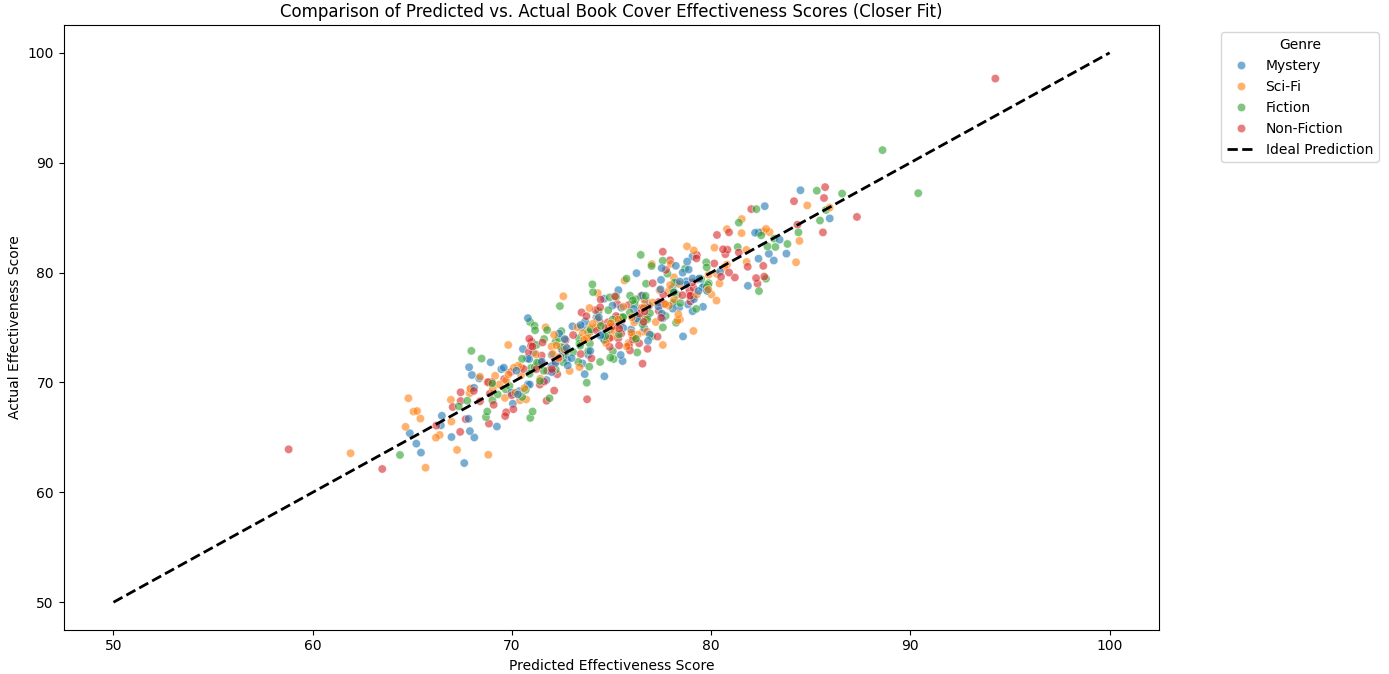
\includegraphics[width=1\textwidth]{Name-Step-3-fig}
            \end{column}
        \end{columns}
        \bigskip
        The consequences of utilizing this analysis lead to strategically optimized book covers, enhancing initial reader engagement and potentially increasing sales.
    \end{frame}
\end{document}